% Options for packages loaded elsewhere
\PassOptionsToPackage{unicode}{hyperref}
\PassOptionsToPackage{hyphens}{url}
\PassOptionsToPackage{dvipsnames,svgnames,x11names}{xcolor}
\documentclass[
  11pt,
]{article}
\usepackage{xcolor}
\usepackage[margin=2cm]{geometry}
\usepackage{amsmath,amssymb}
\setcounter{secnumdepth}{-\maxdimen} % remove section numbering
\usepackage{iftex}
\ifPDFTeX
  \usepackage[T1]{fontenc}
  \usepackage[utf8]{inputenc}
  \usepackage{textcomp} % provide euro and other symbols
\else % if luatex or xetex
  \usepackage{unicode-math} % this also loads fontspec
  \defaultfontfeatures{Scale=MatchLowercase}
  \defaultfontfeatures[\rmfamily]{Ligatures=TeX,Scale=1}
\fi
\usepackage{lmodern}
\ifPDFTeX\else
  % xetex/luatex font selection
    \setmonofont[Scale=0.8,BoldFont=DejaVuSansMono-Bold.ttf]{DejaVuSansMono.ttf}
\fi
% Use upquote if available, for straight quotes in verbatim environments
\IfFileExists{upquote.sty}{\usepackage{upquote}}{}
\IfFileExists{microtype.sty}{% use microtype if available
  \usepackage[]{microtype}
  \UseMicrotypeSet[protrusion]{basicmath} % disable protrusion for tt fonts
}{}
\makeatletter
\@ifundefined{KOMAClassName}{% if non-KOMA class
  \IfFileExists{parskip.sty}{%
    \usepackage{parskip}
  }{% else
    \setlength{\parindent}{0pt}
    \setlength{\parskip}{6pt plus 2pt minus 1pt}}
}{% if KOMA class
  \KOMAoptions{parskip=half}}
\makeatother
\usepackage{graphicx}
\makeatletter
\newsavebox\pandoc@box
\newcommand*\pandocbounded[1]{% scales image to fit in text height/width
  \sbox\pandoc@box{#1}%
  \Gscale@div\@tempa{\textheight}{\dimexpr\ht\pandoc@box+\dp\pandoc@box\relax}%
  \Gscale@div\@tempb{\linewidth}{\wd\pandoc@box}%
  \ifdim\@tempb\p@<\@tempa\p@\let\@tempa\@tempb\fi% select the smaller of both
  \ifdim\@tempa\p@<\p@\scalebox{\@tempa}{\usebox\pandoc@box}%
  \else\usebox{\pandoc@box}%
  \fi%
}
% Set default figure placement to htbp
\def\fps@figure{htbp}
\makeatother
\ifLuaTeX
\usepackage[bidi=basic]{babel}
\else
\usepackage[bidi=default]{babel}
\fi
\babelprovide[main,import]{french}
% get rid of language-specific shorthands (see #6817):
\let\LanguageShortHands\languageshorthands
\def\languageshorthands#1{}
\setlength{\emergencystretch}{3em} % prevent overfull lines
\providecommand{\tightlist}{%
  \setlength{\itemsep}{0pt}\setlength{\parskip}{0pt}}
% Ajouté au préambule de chaque document par generer.sh
\usepackage{xcolor}
\usepackage{newunicodechar}
\newfontfamily\symbolfont{DejaVuSans.ttf}
% Caractères absents de Latin Modern (flèches, comparateurs, cases) : repli sur DejaVu Sans
\newunicodechar{→}{{\symbolfont →}}
\newunicodechar{←}{{\symbolfont ←}}
\newunicodechar{⇄}{{\symbolfont ⇄}}
\newunicodechar{↔}{{\symbolfont ↔}}
\newunicodechar{≥}{{\symbolfont ≥}}
\newunicodechar{≤}{{\symbolfont ≤}}
\newunicodechar{≠}{{\symbolfont ≠}}
\newunicodechar{≈}{{\symbolfont ≈}}
\newunicodechar{✓}{{\symbolfont ✓}}
\newunicodechar{✗}{{\symbolfont ✗}}
\newunicodechar{⚠}{{\symbolfont ⚠}}
\newunicodechar{✅}{{\symbolfont\color[rgb]{0.1,0.55,0.2}✔}}
\newunicodechar{‑}{\mbox{-}}
% Retour à la ligne dans les blocs de code et les URL longues
\usepackage{fvextra}
\DefineVerbatimEnvironment{Highlighting}{Verbatim}{breaklines,commandchars=\\\{\}}
\usepackage{xurl}
\setlength{\emergencystretch}{3em}
\AtBeginEnvironment{longtable}{\small}
% Figures flottantes (pas de demi-pages vides), jamais plus hautes que 85 % de la page
\usepackage{float}
\floatplacement{figure}{htbp}
\usepackage{adjustbox}
\providecommand*\pandocbounded[1]{#1}% absent des documents sans image
\renewcommand*\pandocbounded[1]{\adjustbox{max width=\linewidth,max totalheight=0.85\textheight}{#1}}
\usepackage[font=small,labelfont=bf]{caption}
% Contenu sur une nouvelle page après la table des matières
\let\tdmorigine\tableofcontents
\renewcommand{\tableofcontents}{\tdmorigine\newpage}
\usepackage{fancyhdr}
\pagestyle{fancy}
\fancyhf{}
\fancyhead[L]{\small SmartRecruit — Qualité logicielle ISO/IEC 25010}
\fancyhead[R]{\small\thepage}
\renewcommand{\headrulewidth}{0.4pt}
\usepackage{bookmark}
\IfFileExists{xurl.sty}{\usepackage{xurl}}{} % add URL line breaks if available
\urlstyle{same}
\hypersetup{
  pdftitle={Diagrammes --- SmartRecruit (Mermaid)},
  pdflang={fr},
  colorlinks=true,
  linkcolor={Maroon},
  filecolor={Maroon},
  citecolor={Blue},
  urlcolor={Blue},
  pdfcreator={LaTeX via pandoc}}

\title{Diagrammes --- SmartRecruit (Mermaid)}
\author{}
\date{}

\begin{document}
\maketitle

\renewcommand*\contentsname{Table des matières}
{
\hypersetup{linkcolor=}
\setcounter{tocdepth}{3}
\tableofcontents
}
Diagrammes du \href{RAPPORT_CONCEPTION.pdf}{rapport de conception}, au
format Mermaid : GitHub les affiche directement. Versions PNG (intégrées
au rapport) : \href{../images/}{\texttt{images/}}, régénérées par
\texttt{bash\ docs/}\allowbreak{}\texttt{qualite/}\allowbreak{}\texttt{latex/}\allowbreak{}\texttt{generer.}\allowbreak{}\texttt{sh}.

\section{1. Cas d\textquotesingle utilisation par
rôle}\label{1-cas-dutilisation-par-ruxf4le}

\pandocbounded{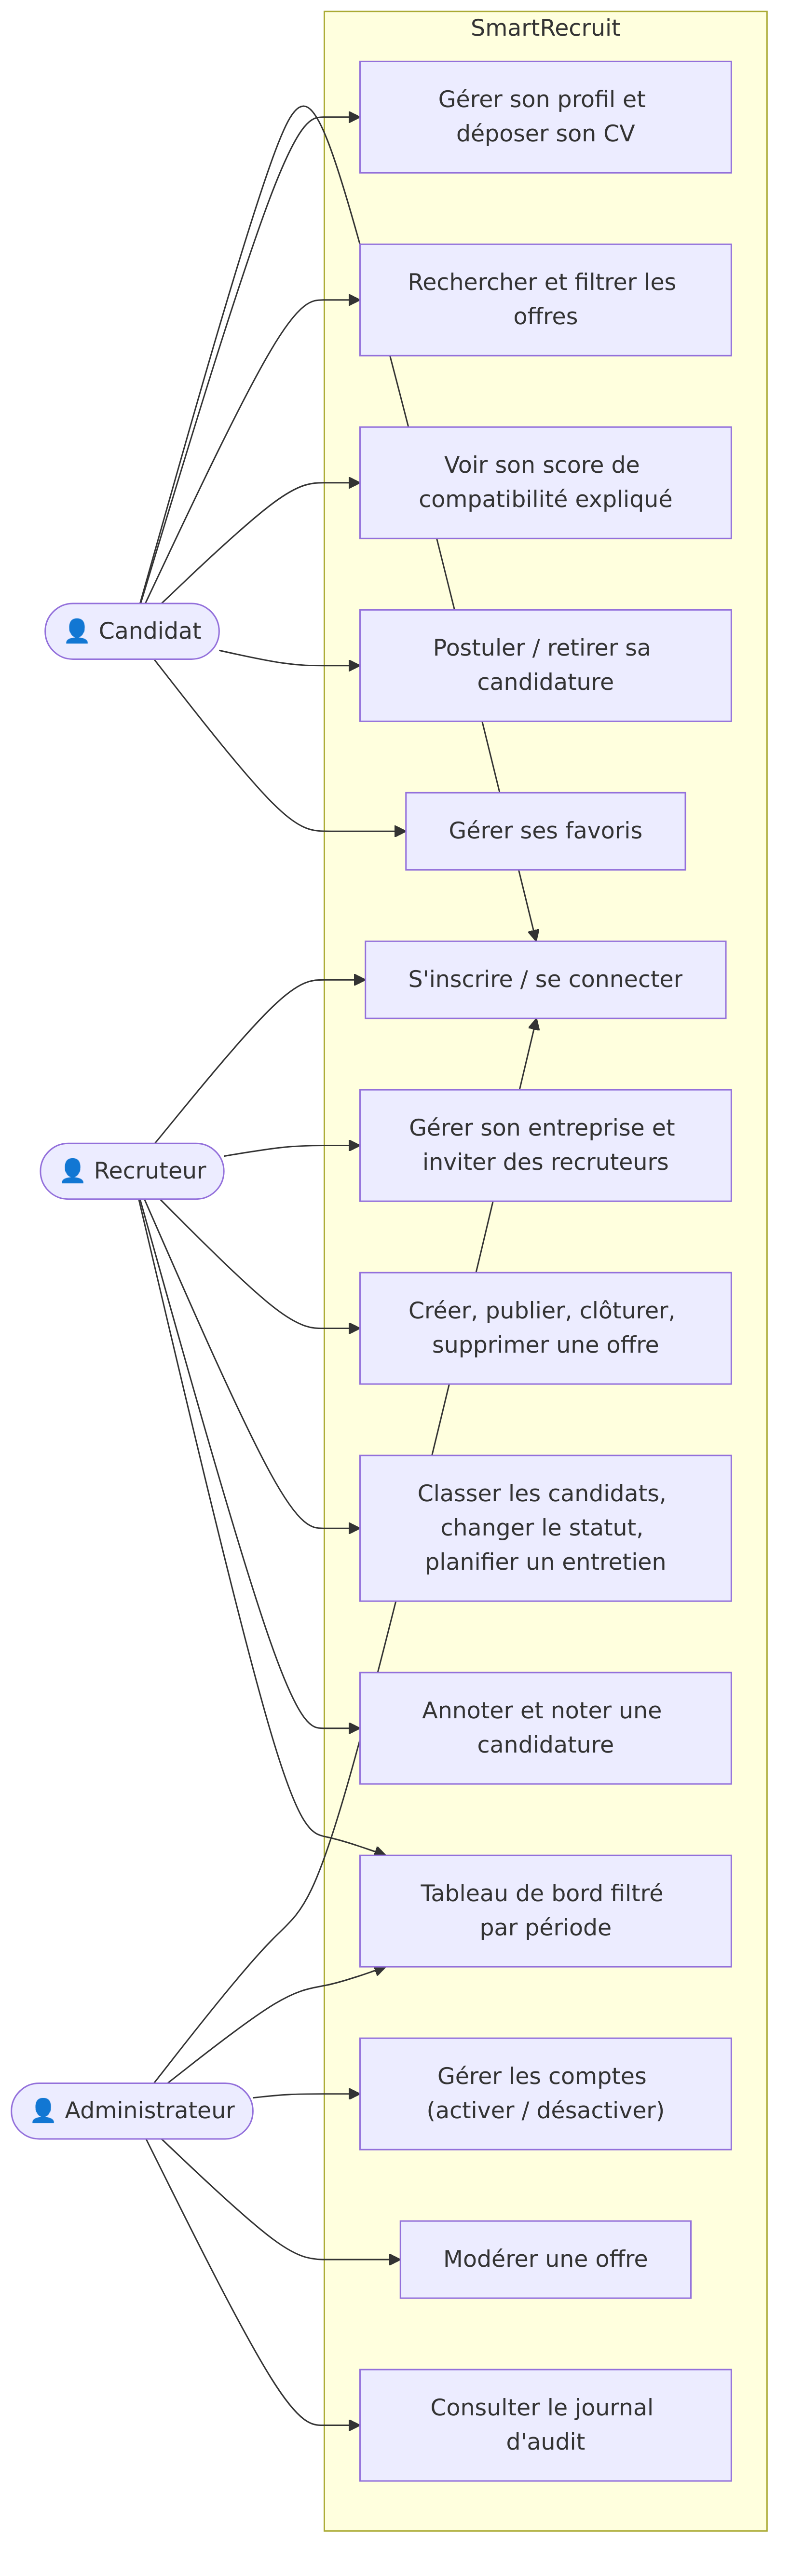
\includegraphics[keepaspectratio]{../images/diagramme-1.png}}

\section{2. Architecture}\label{2-architecture}

\pandocbounded{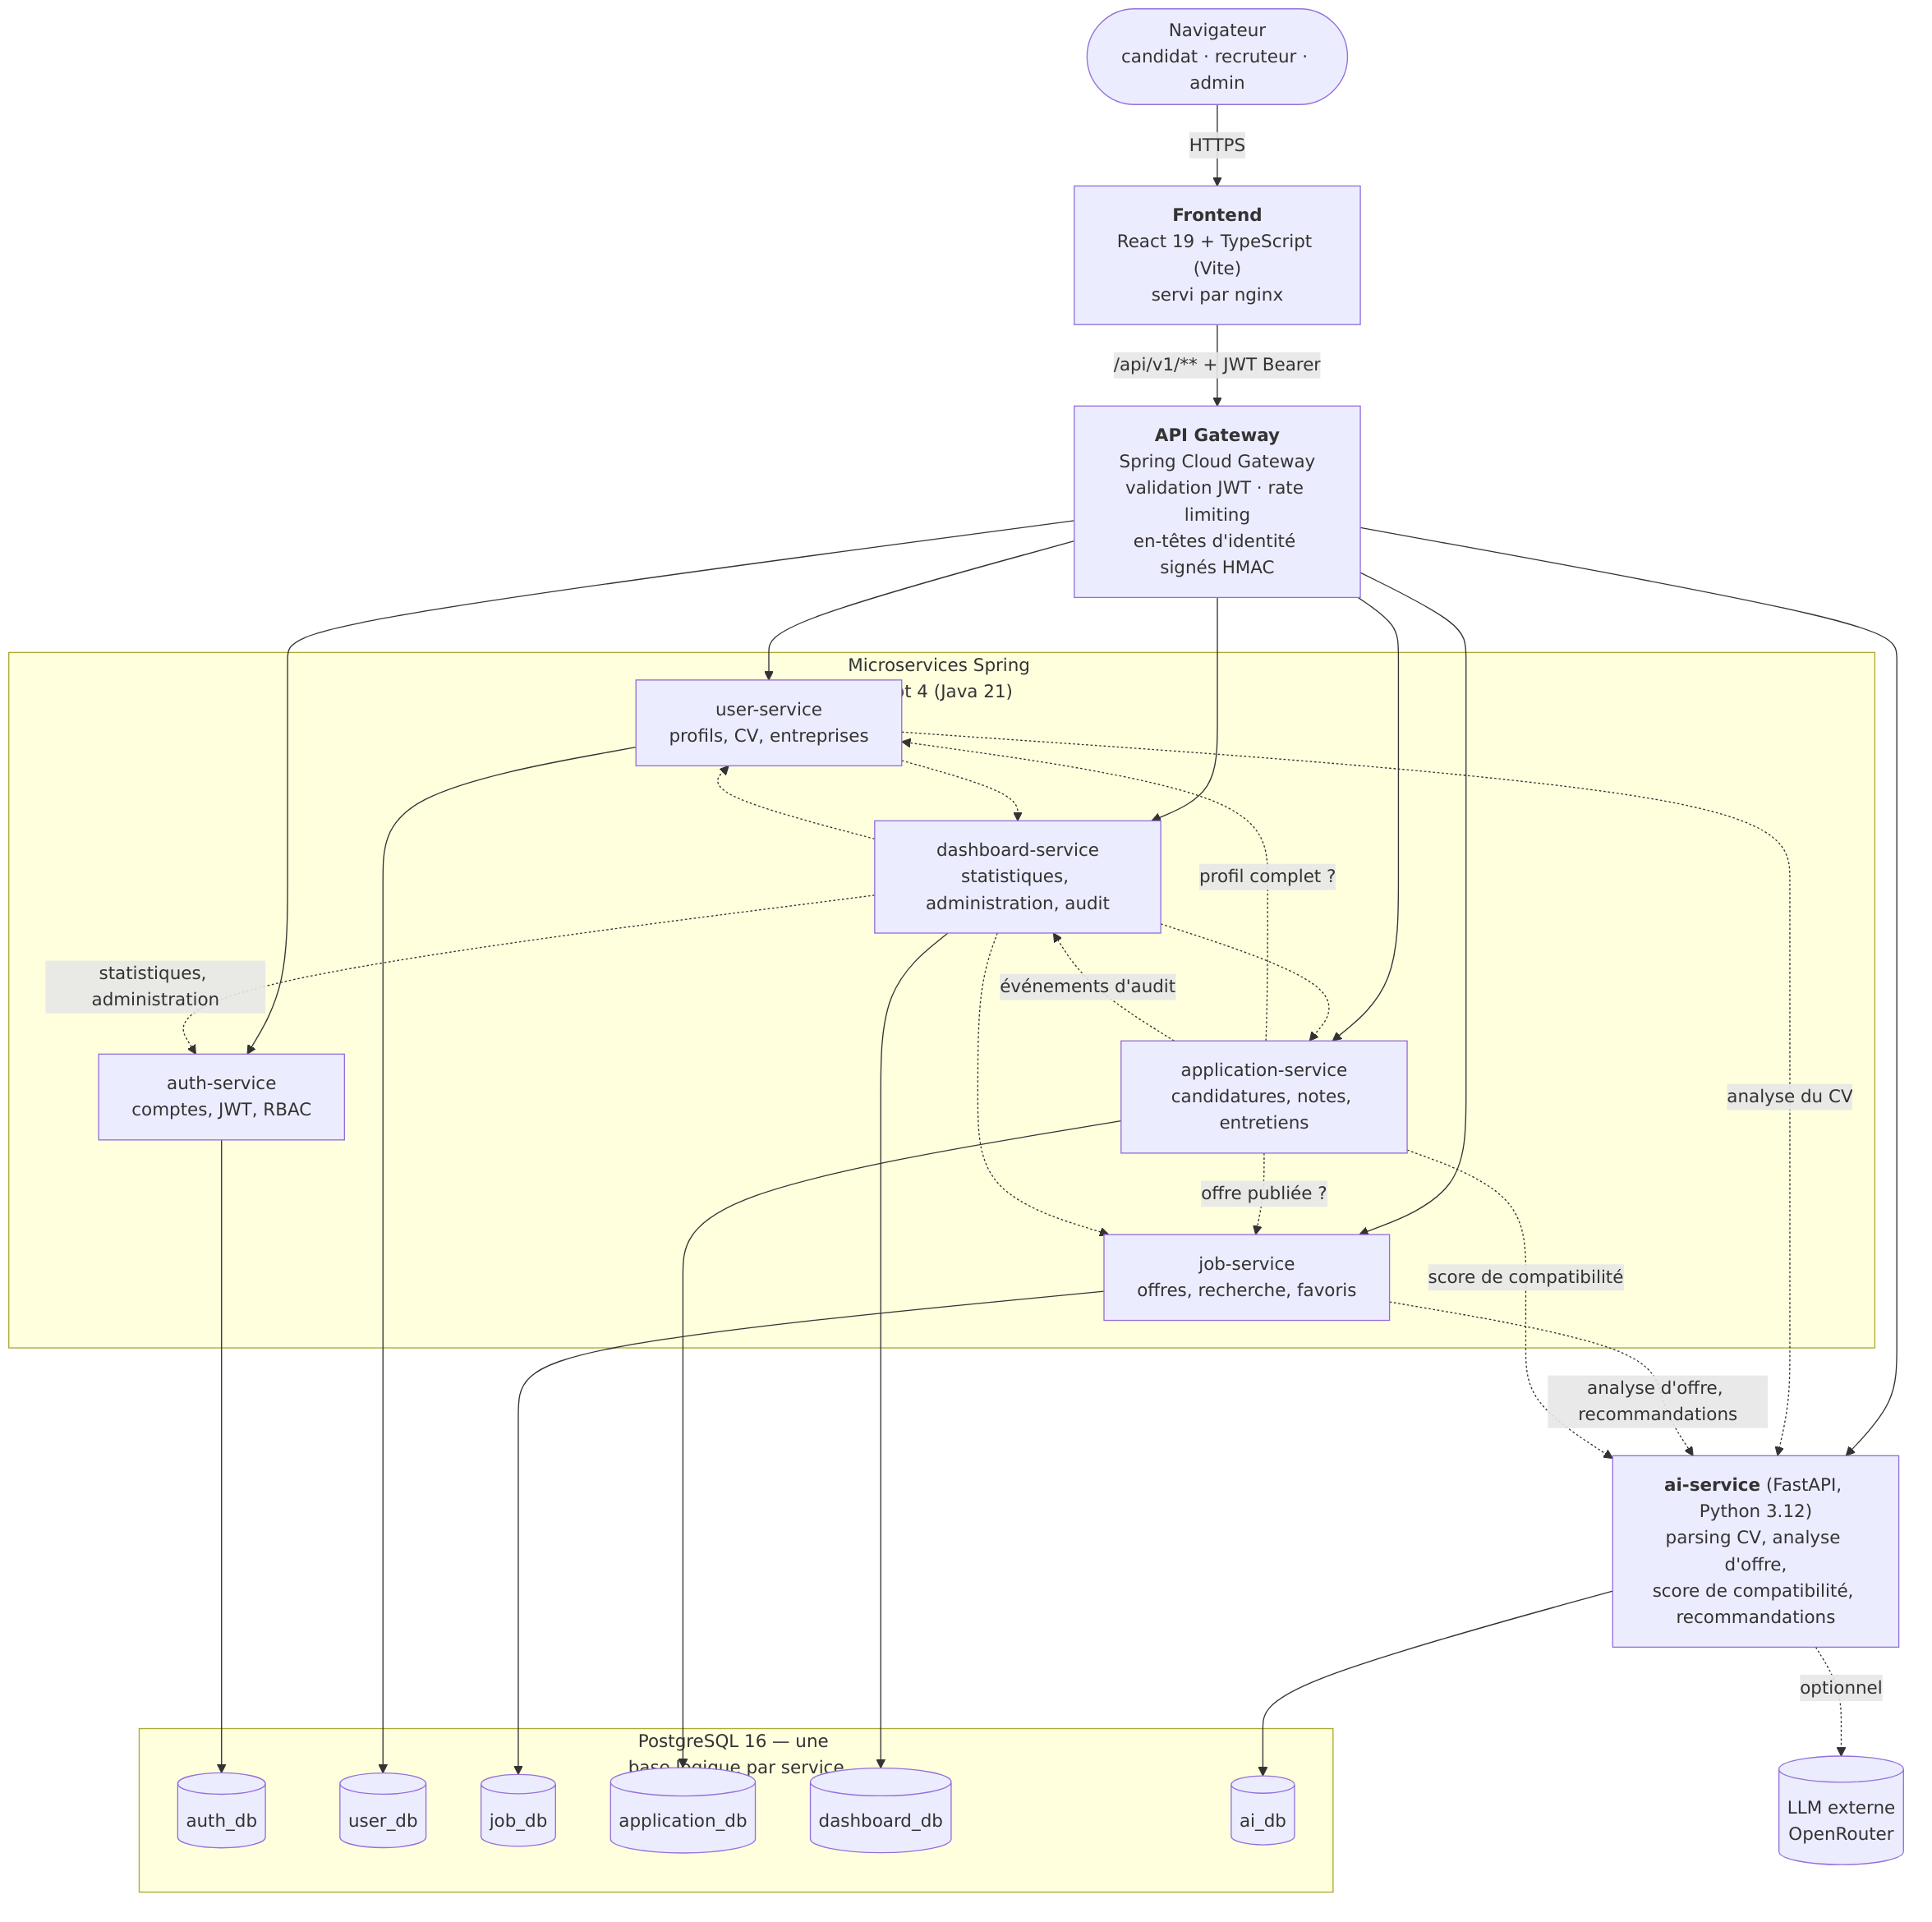
\includegraphics[keepaspectratio]{../images/diagramme-2.png}}

\section{3. Modèle de données}\label{3-moduxe8le-de-donnuxe9es}

\pandocbounded{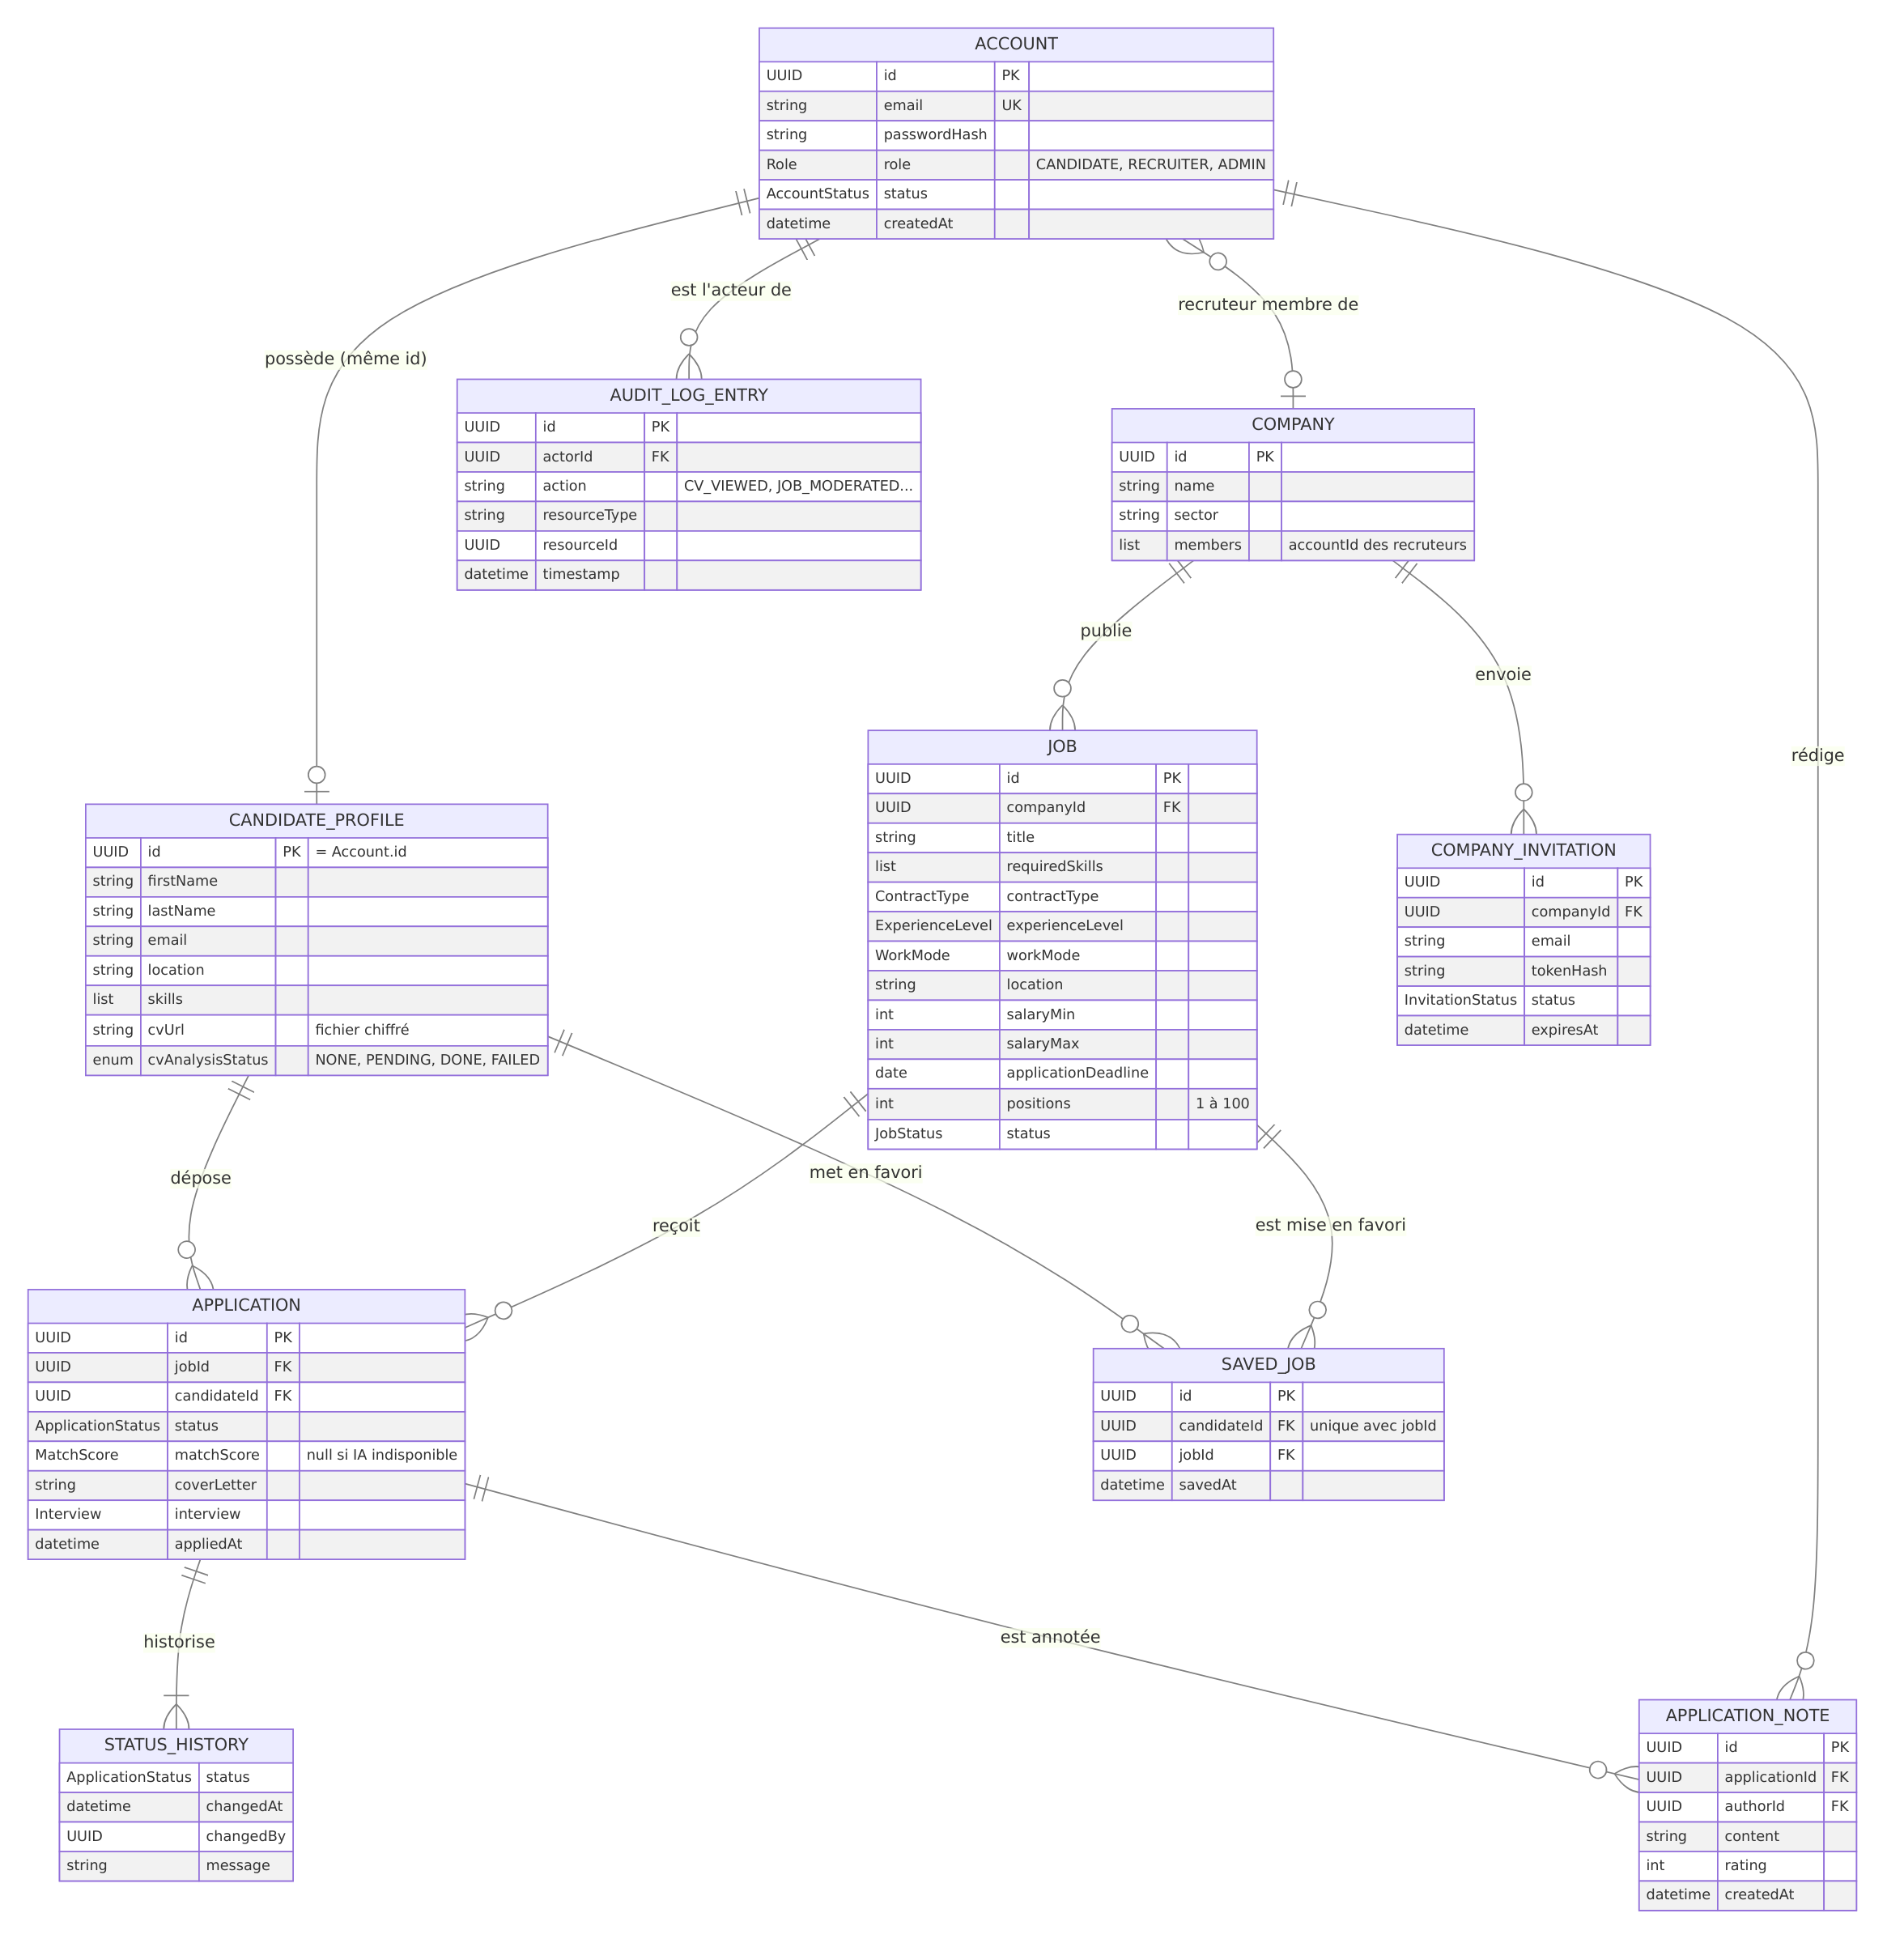
\includegraphics[keepaspectratio]{../images/diagramme-3.png}}

Entre microservices, les clés étrangères sont \textbf{logiques} (chaque
service possède sa base).

\section{4. Workflow d\textquotesingle une candidature
(RG‑03)}\label{4-workflow-dune-candidature-rg03}

\pandocbounded{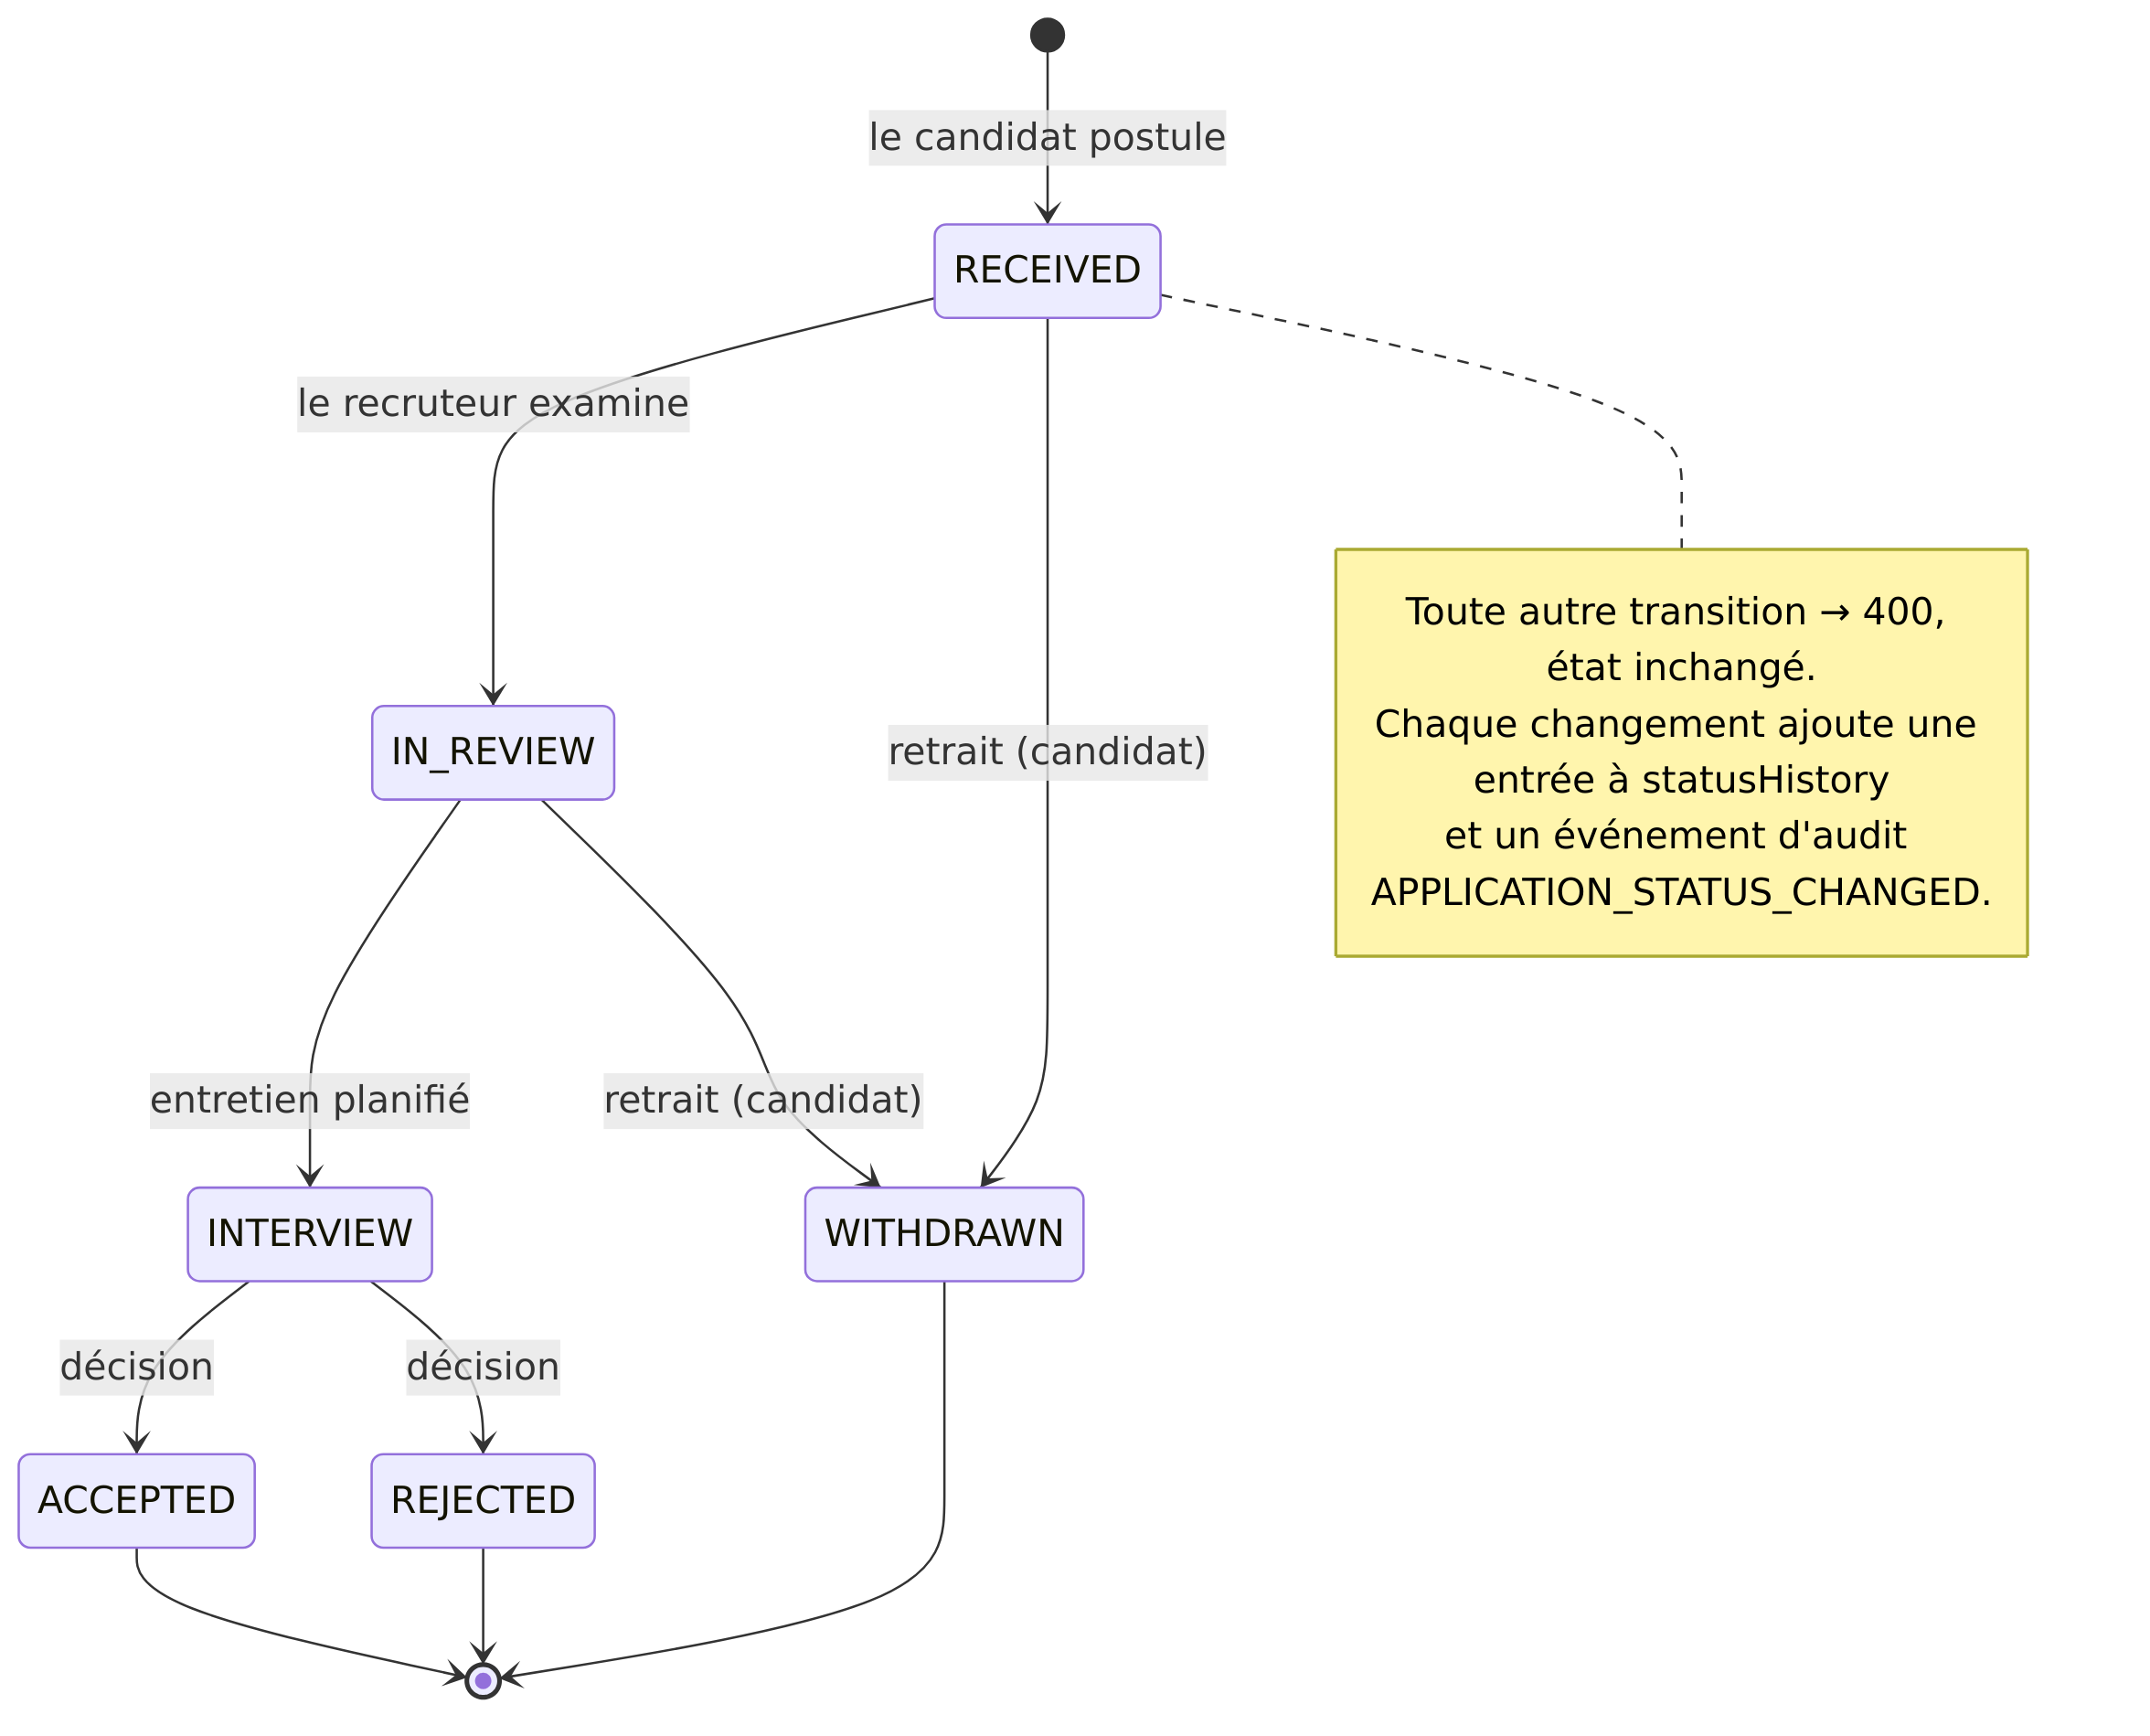
\includegraphics[keepaspectratio]{../images/diagramme-4.png}}

\section{5. Workflow d\textquotesingle une offre (RG‑08,
RG‑09)}\label{5-workflow-dune-offre-rg08-rg09}

\pandocbounded{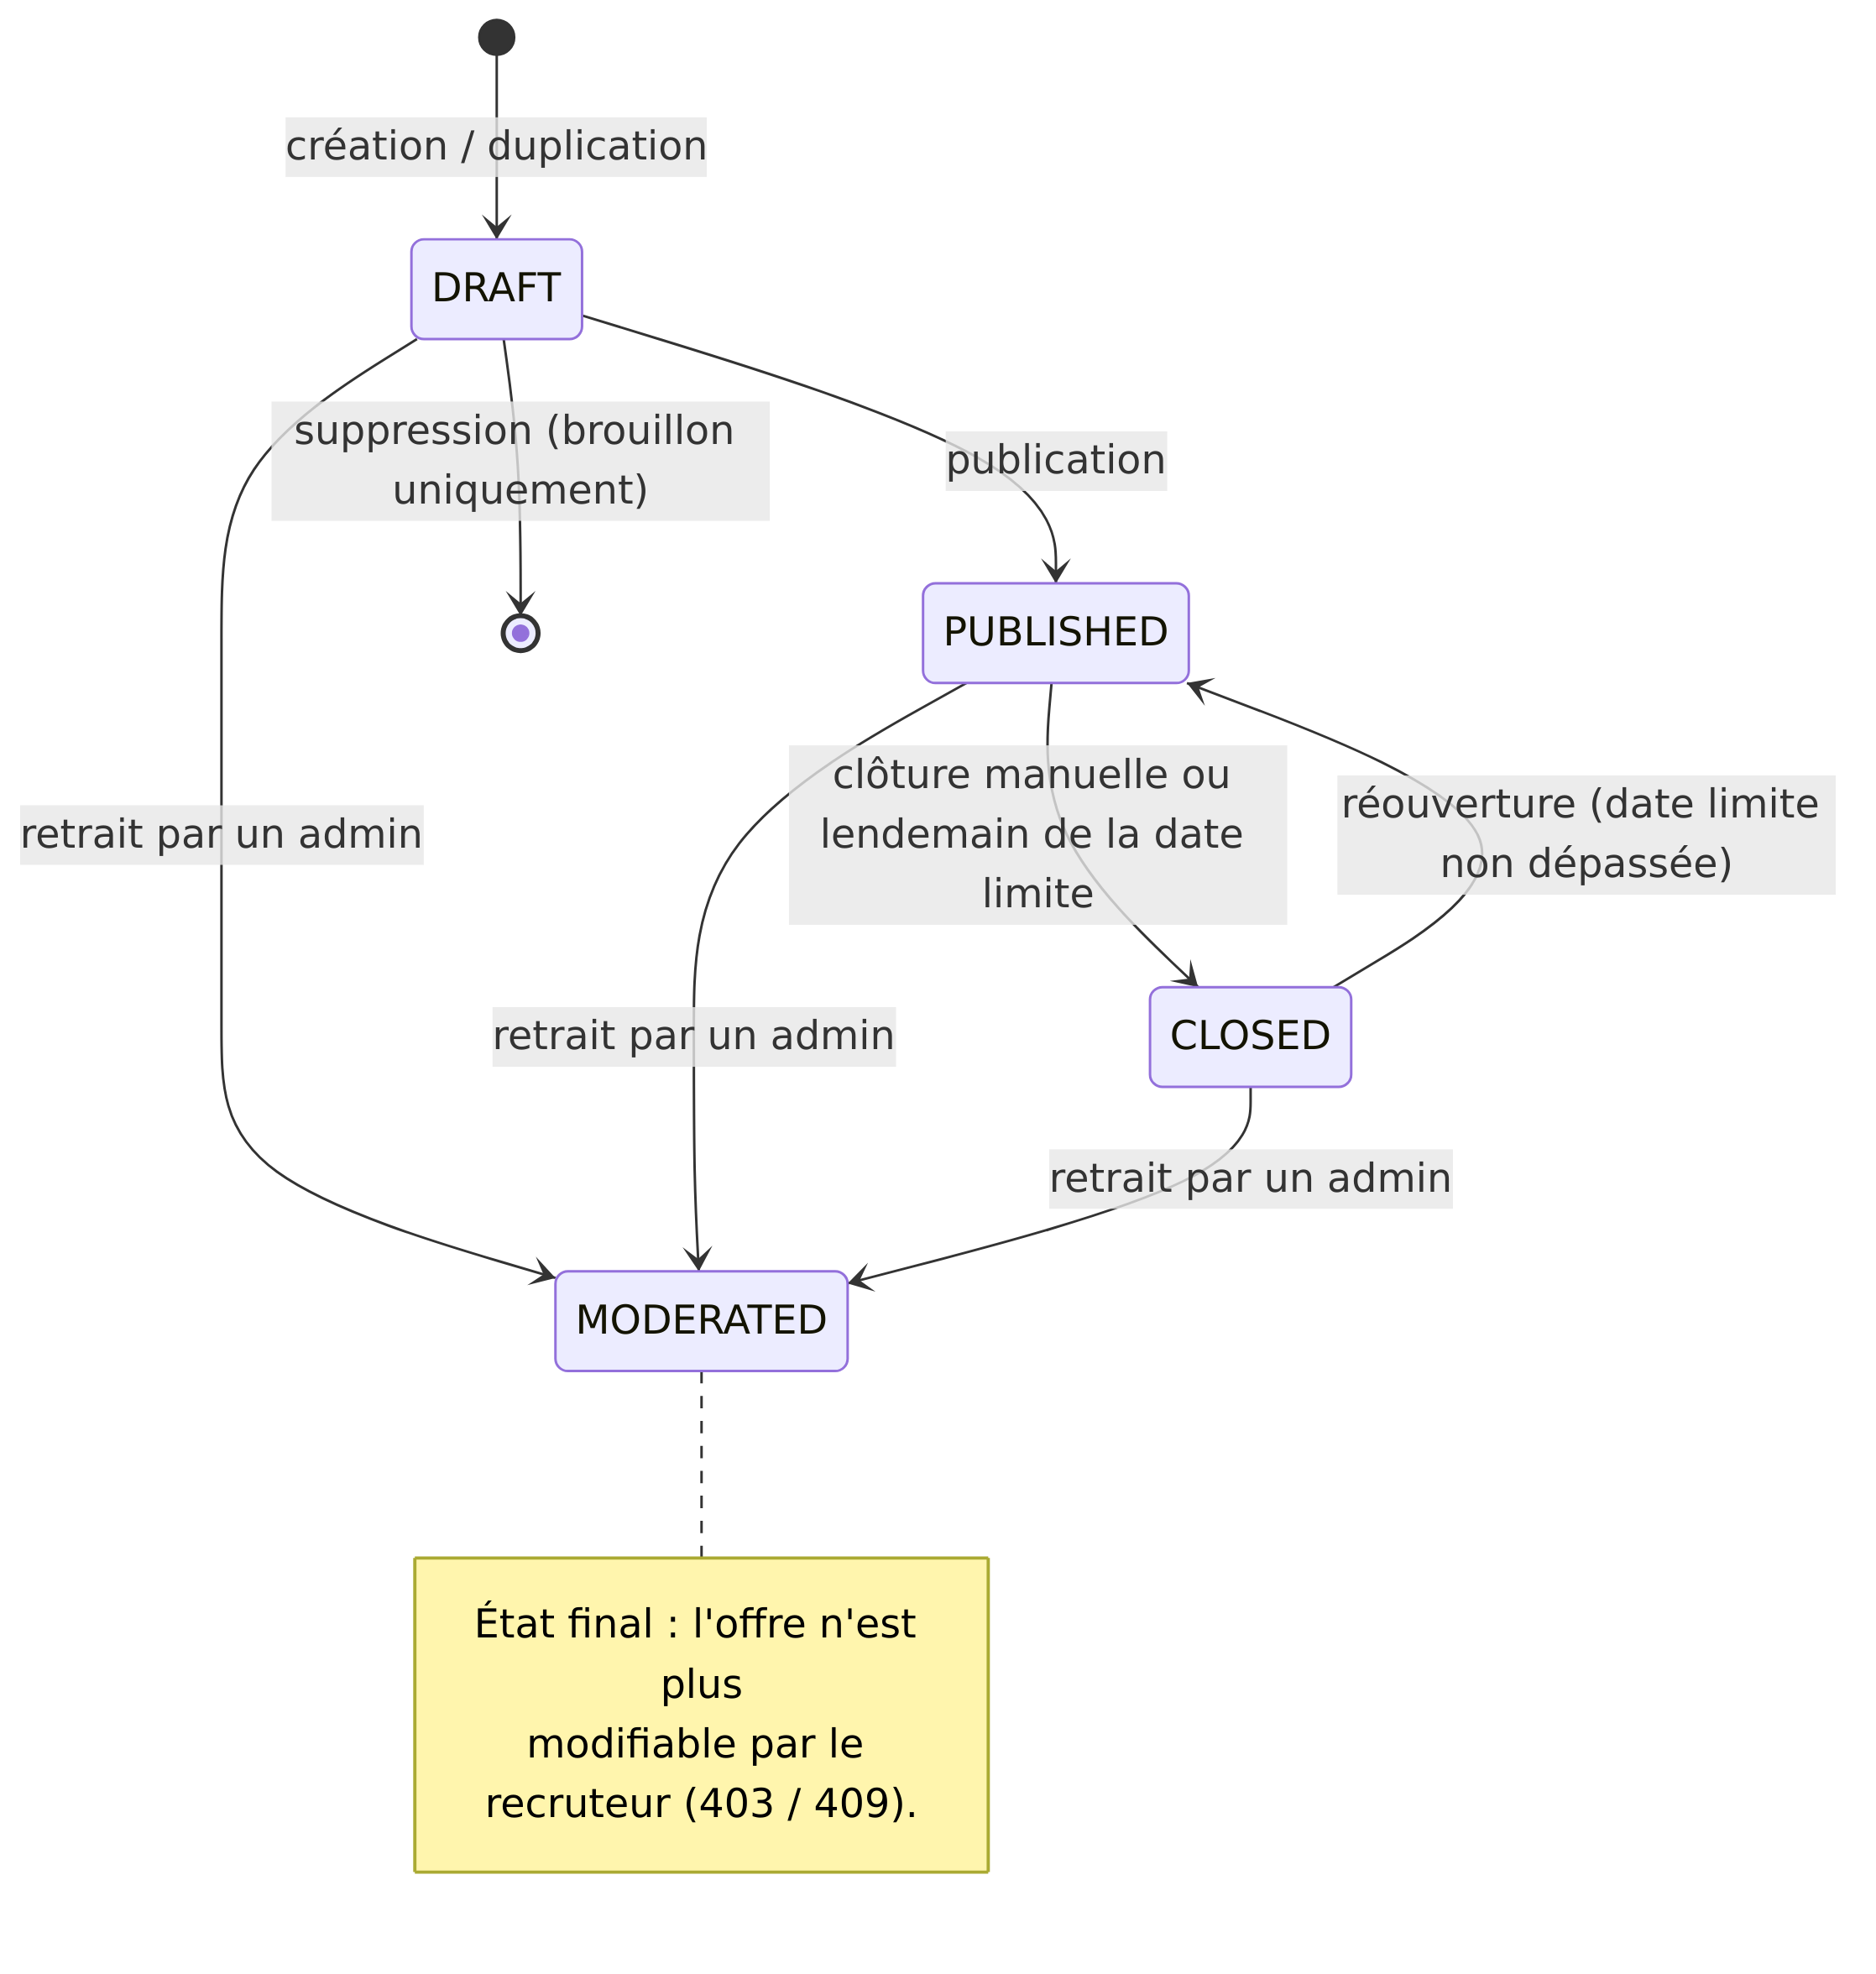
\includegraphics[keepaspectratio]{../images/diagramme-5.png}}

\section{6. Séquence : postuler à une
offre}\label{6-suxe9quence--postuler-uxe0-une-offre}

\pandocbounded{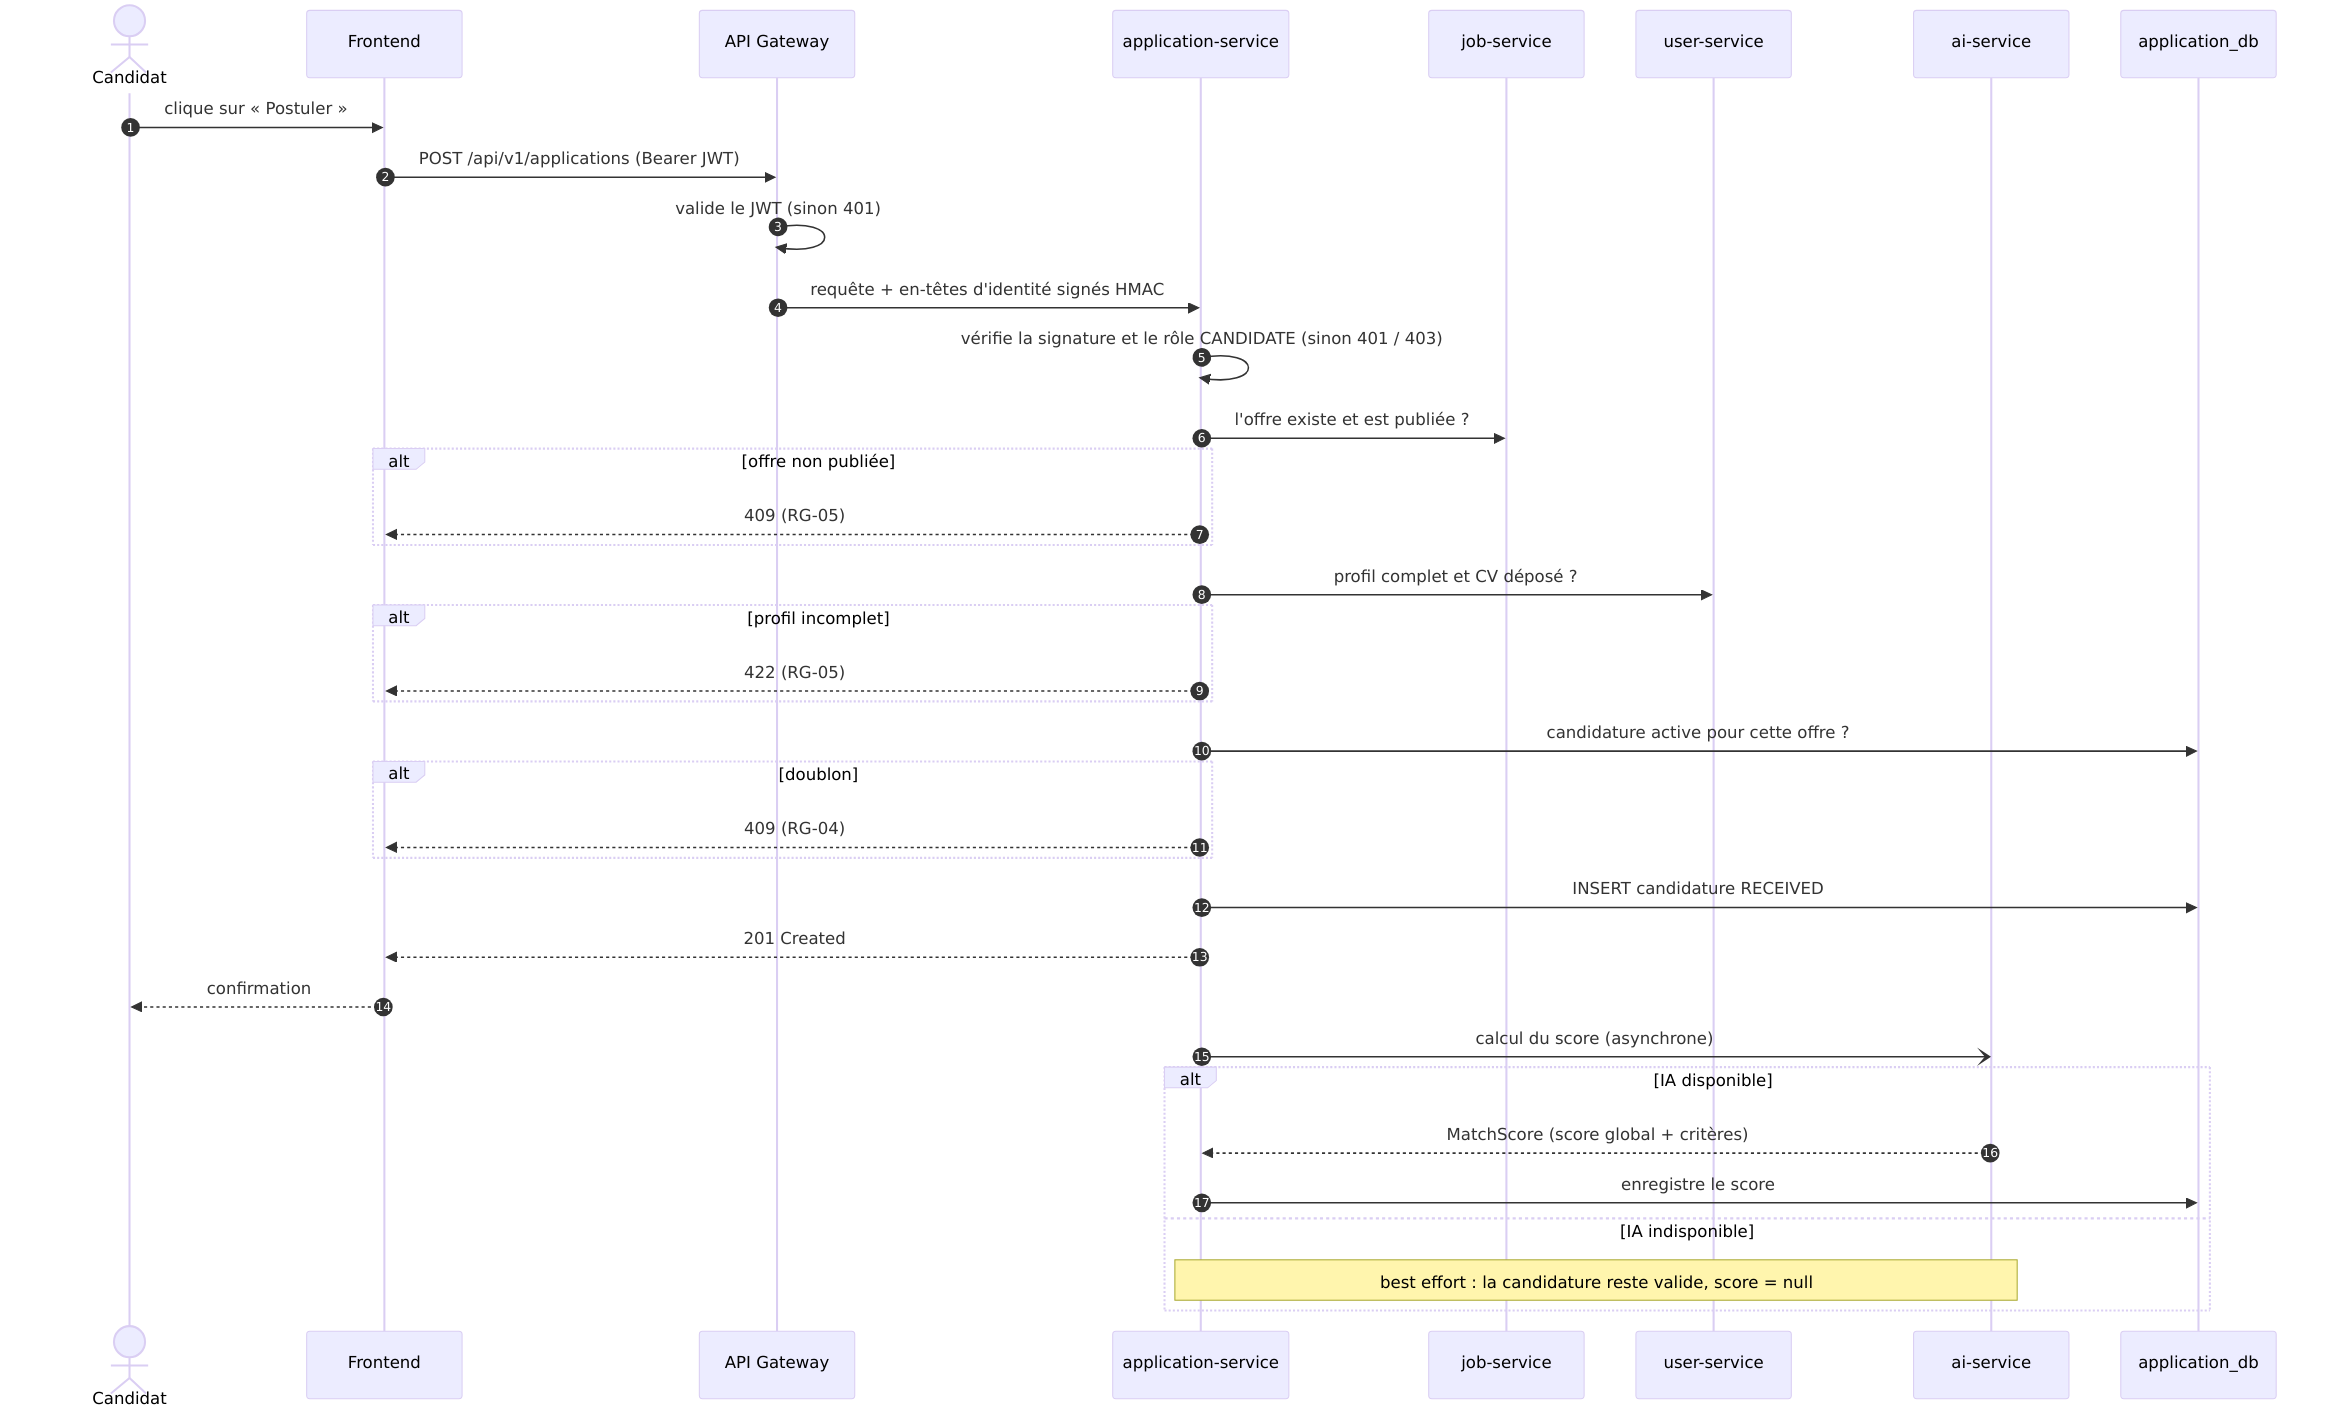
\includegraphics[keepaspectratio]{../images/diagramme-6.png}}

\section{7. Stratégie de test : couches → outils → caractéristiques
ISO/IEC
25010}\label{7-stratuxe9gie-de-test--couches--outils--caractuxe9ristiques-isoiec-25010}

\pandocbounded{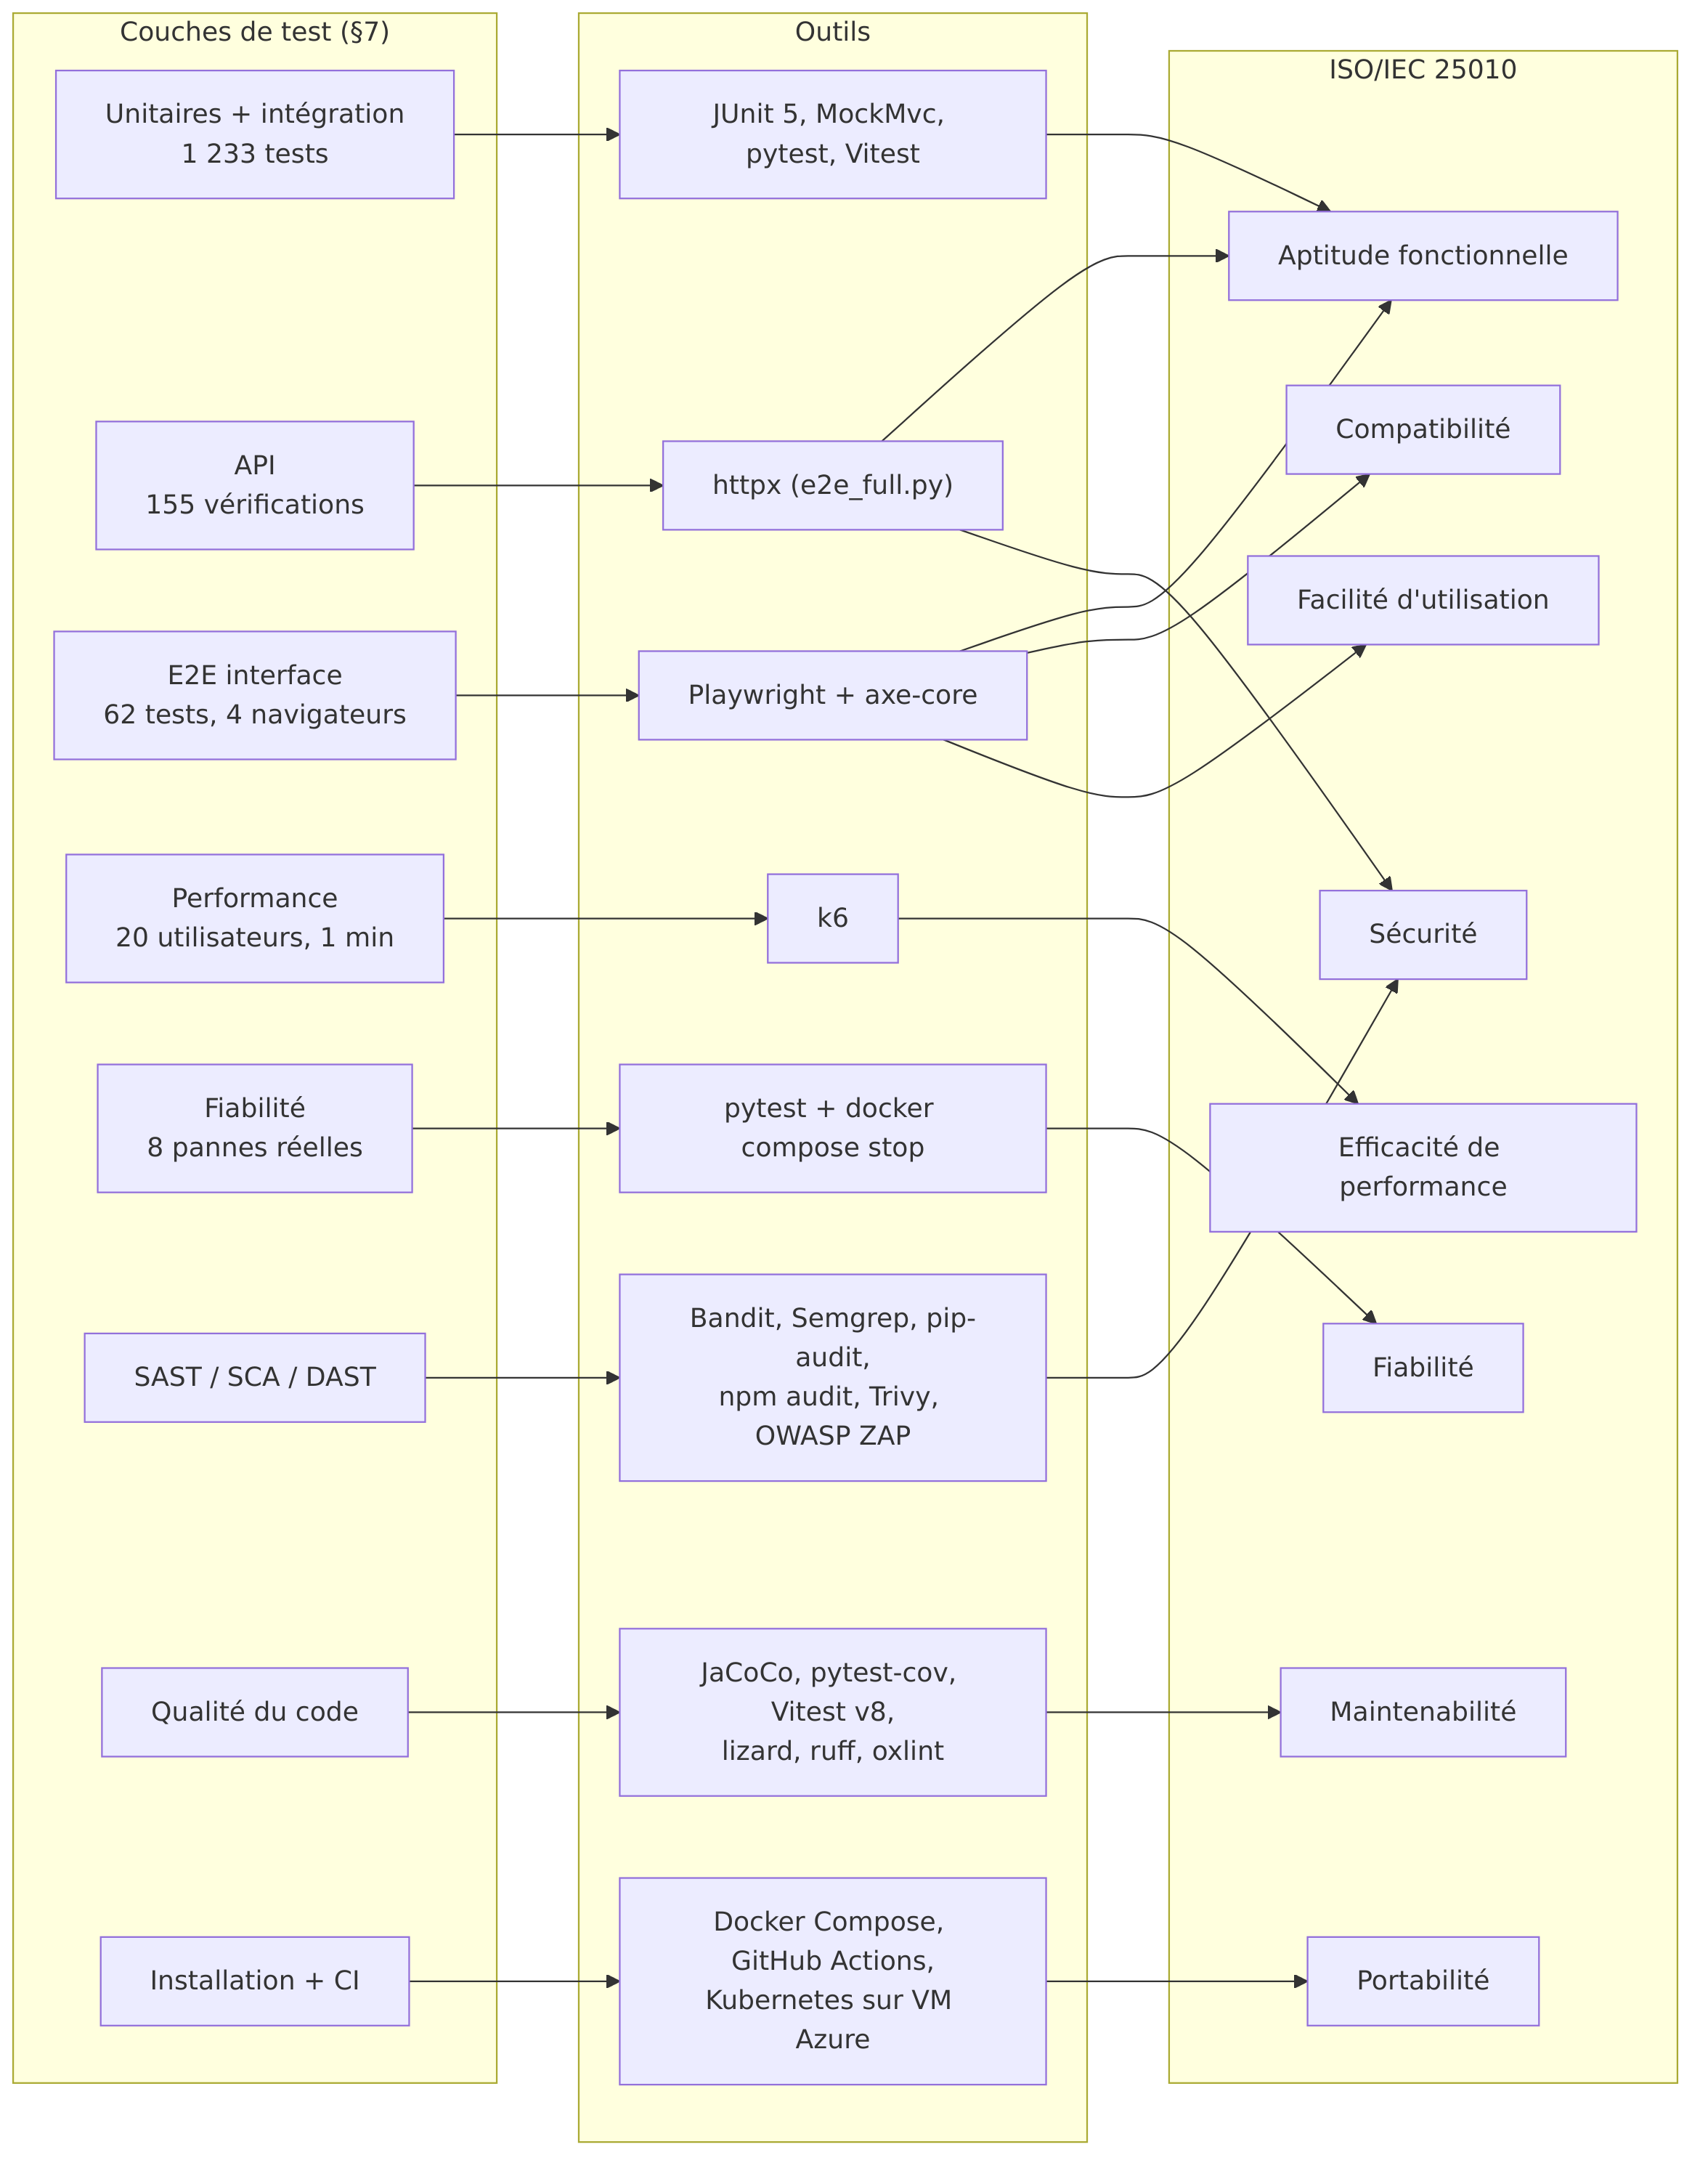
\includegraphics[keepaspectratio]{../images/diagramme-7.png}}

\section{8. Pipeline CI/CD (GitHub
Actions)}\label{8-pipeline-cicd-github-actions}

\pandocbounded{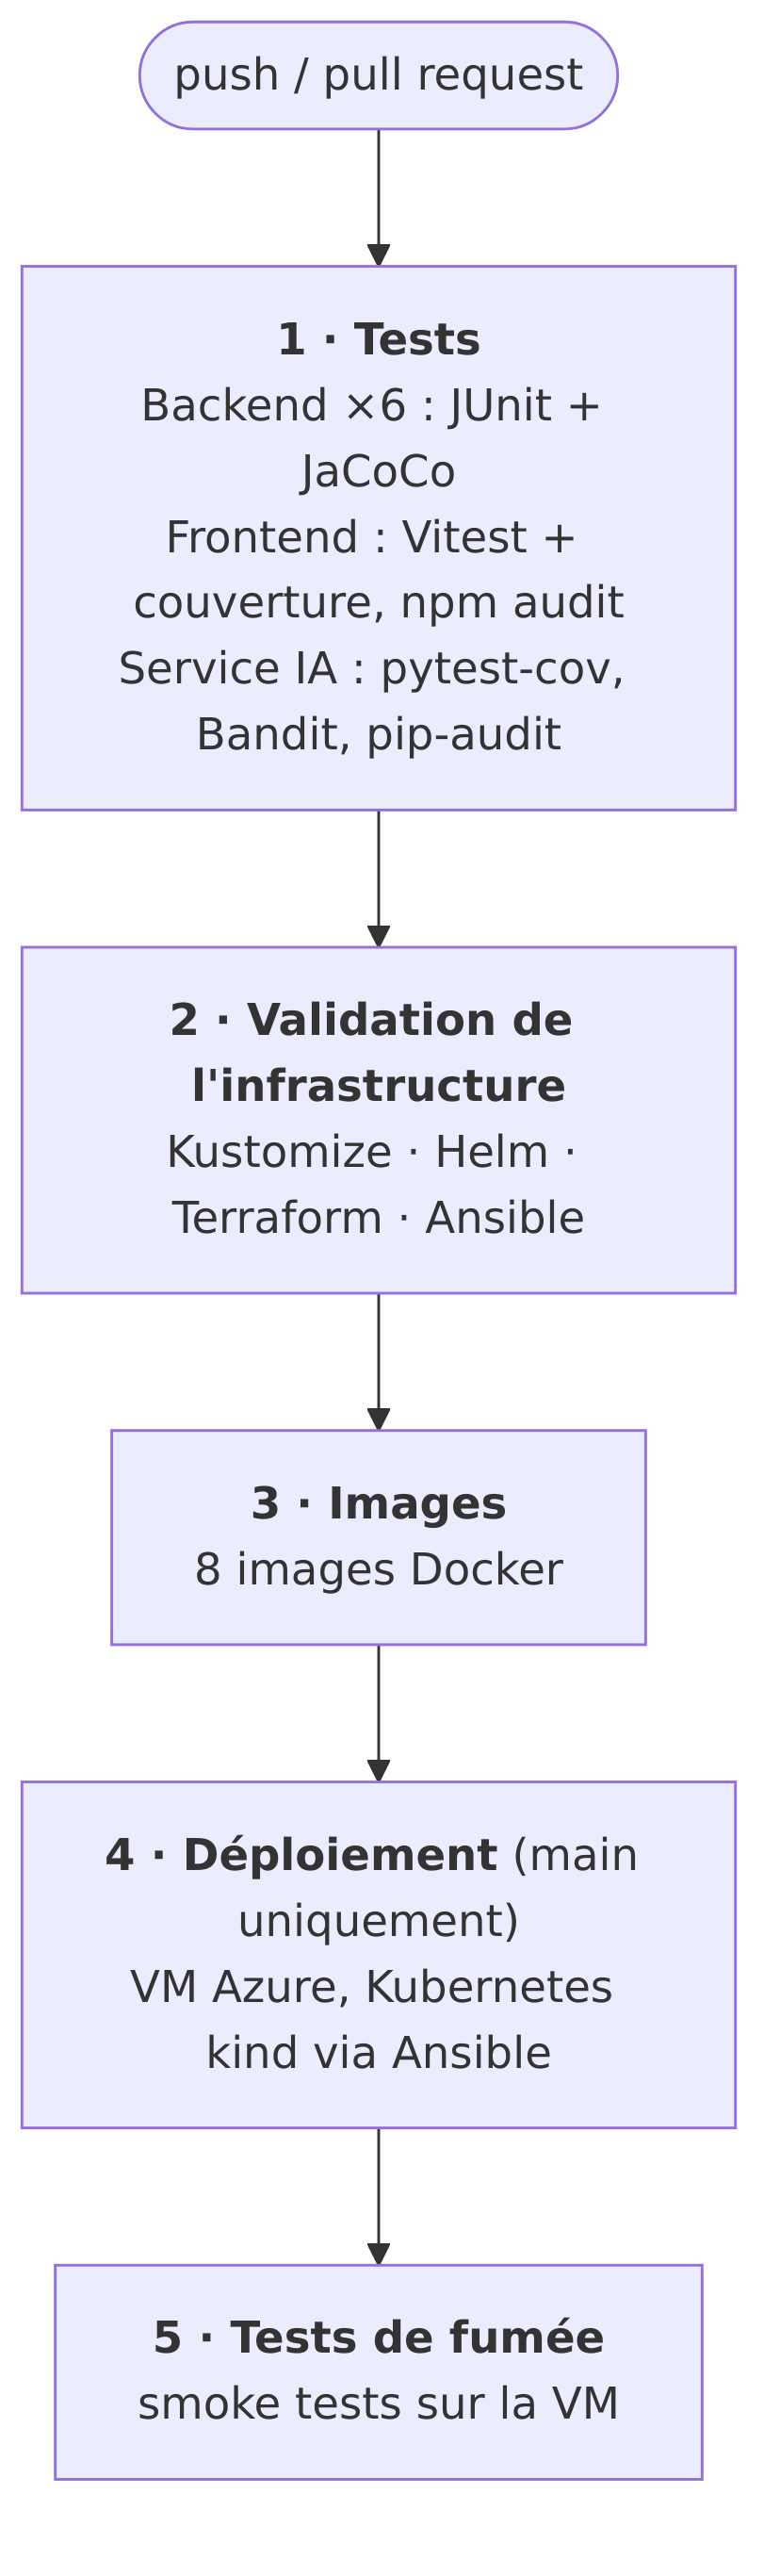
\includegraphics[keepaspectratio]{../images/diagramme-8.png}}

\end{document}
